\begin{center}
\begin{minipage}{\linewidth}\centering
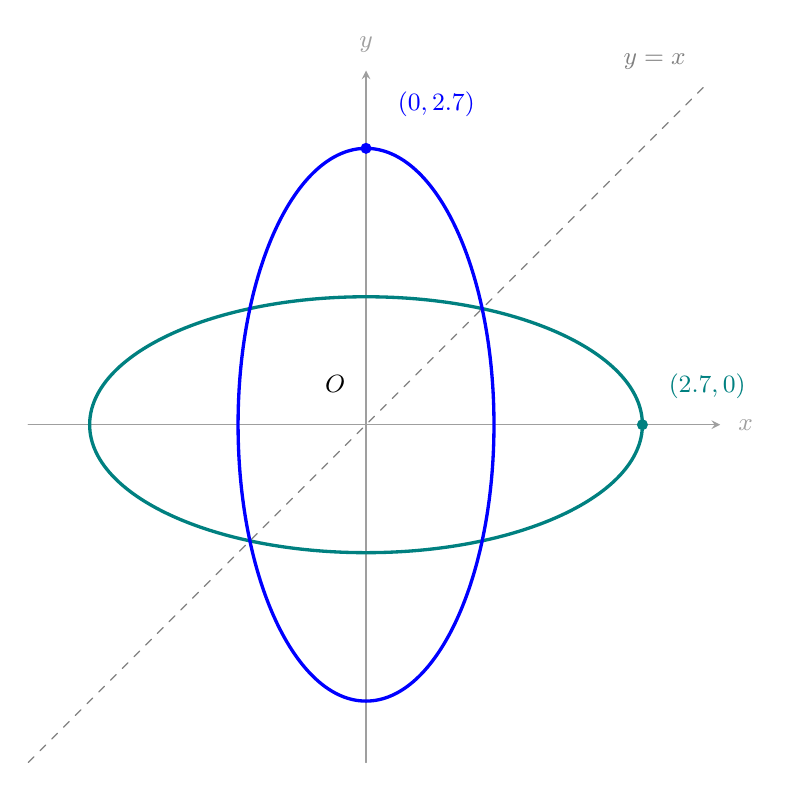
\begin{tikzpicture}[x=1.3cm,y=1.3cm,>=stealth,font=\small,line cap=round,line join=round]
\draw[->,gray!75] (-3.3,0)--(3.46,0) node[right=3pt]{$x$};
\draw[->,gray!75] (0,-3.3)--(0,3.46) node[above=3pt]{$y$};
\node at (-.3,.4) {$O$};
\draw[gray,dashed] (-3.3,-3.3)--(3.3,3.3) node[above left=3pt]{$y=x$};

\draw[teal,very thick] (0,0) ellipse (2.7 and 1.25);
\draw[blue,very thick] (0,0) ellipse (1.25 and 2.7);
\fill[teal] (2.7,0) circle(2pt) node[above right=6pt]{$(2.7,0)$};
\fill[blue] (0,2.7) circle(2pt) node[above right=8pt]{$(0,2.7)$};

\end{tikzpicture}\par\smallskip
{\small \textcolor{teal}{\rule[.5ex]{1em}{.8pt}\ $x^2/2.7^2+y^2/1.25^2=1$}\qquad\textcolor{blue}{\rule[.5ex]{1em}{.8pt}\ $y^2/2.7^2+x^2/1.25^2=1$}}\par
{\small 椭圆的长、短轴交换，半轴长度不变。}\par\smallskip
\end{minipage}
\end{center}
